\documentclass[11pt]{scrartcl}
\usepackage[utf8]{inputenc}
\usepackage{mathtools}
\usepackage{amssymb}
\usepackage{fancyhdr}
\usepackage{answers}
\usepackage{lastpage}
\usepackage{datetime}
\usepackage{titlesec}
\usepackage{makeidx}
\usepackage{graphicx}
\graphicspath{ {./images/} }
\usepackage{bm}
\usepackage{evan}[fancy, sexy, hdr, colorsec]
\usepackage[dvipsnames]{xcolor}
\usepackage[margin = 1in, letterpaper, portrait]{geometry}
\usepackage[version = 4]{mhchem}

\everymath{\displaystyle}

\pagestyle{fancy}
\rhead{Last Updated: \today}
\lhead{Kinematics Problem Set}
\cfoot{Page \thepage\ of \pageref*{LastPage}}

\renewcommand*\contentsname{\S Table of Contents}

\makeindex


\begin{document}

\titleformat{\section}{\normalfont\Large\bfseries}{\color{red}\S \thesection}{0.5em}{}
\titleformat{\subsection}{\normalfont\Large\bfseries}{\color{olive}\S \thesubsection}{0.5em}{}
\titleformat{\subsubsection}{\normalfont\Large\bfseries}{\color{blue}\S \thesubsubsection}{0.5em}{}

\begin{center}
    \Large \textbf{Kinematics Problem Set}
\end{center}
\begin{center}
    \Large Rajeev Atla
\end{center}

\begin{itemize}
    \item Problem weights
    \begin{itemize}
        \item Problem $n$ is worth $n$ points
        \item So problem 1 is worth 1 point, problem 2 is worth 2 points, etc.
        \item Total of 15 points
    \end{itemize}
    \item Try to get as many points as you can!
    \item Dont forget to have fun!
    \item Feel free to reach out for hints
    \item There will be a leaderboard
\end{itemize}

\newpage

\section{Problem 1}
Using calculus and/or geometry, derive the equation

$$
x(t) = x_0 + v_0 t + \frac{1}{2} at^2
$$

\subsection*{Solution}
We go the calculus route.
We know that $v(t) = v_0 + at$ and that $x = \int v(t)\ dt$.
Carrying out the integral using the power rule, we see that

$$
x(t) = C + v_0 t + \frac{1}{2} at^2
$$

Substituting $t = 0$, we see that the constant $C$ must be equal to the intitial value of $x$, recovering the equation.

\newpage

\section{Problem 2}
For two vectors $\bm{a}$ and $\bm{b}$, prove the following inequalities:

$$
|\bm{a}| - |\bm{b}| \leq |\bm{a}+\bm{b}| \leq |\bm{a}|+ |\bm{b}|
$$

\subsection*{Solution}
This problem can actually be done without much algebra.
We consider the wording, which is eerily similar to the triangle inequality.
In fact, its actually the triangle inequality for vectors.

First, lets look at some edge cases.
Suppose both $\bm{a}$ and $\bm{b}$ are vectors in the same direction (parallel), making sort of a degenerate triangle.
Drawing it out, we can see that the two vectors add one dimensionally with a total magnitude of $|\bm{a}|+ |\bm{b}|$.

Another edge case we can consider will be when the two vectors are in opposing directions (known as antiparallel), making yet anothe degenerate triangle.
This means that magnitude of the final vector will be $|\bm{a}| - |\bm{b}|$.

These two edge cases form the equality cases of our inequality.
To complete the proof, we use the cosine rule and see that the inequality holds even in non-edge cases.
Suppose we know the angle between the two vectors to be $\theta$.
The cosine rule states that the magnitude of the sum will obey

$$
|\bm{a}+\bm{b}| = |\bm{a}|^2 + |\bm{b}|^2 - 2|\bm{a}||\bm{b}| \cos{\theta}
$$

Substituting $\theta = \pi$ and $\theta = \frac{\pi}{2}$, we both recover our edge cases and see that the inequality holds true. 

\newpage

\section{Problem 3}
A ball is thrown from the ground.
The ball crosses the height $h_1$ twice, with $T_1$ seconds between crossings.
Above, at a height of $h_2$, the ball takes $T_2$ seconds between crossings.
Derive an expression for $g$, the acceleration due to gravity, in terms of these variables.

\subsection*{Solution}
This is a pretty algebra-heavy problem.
Let the initial velocity of the ball be $v_0$, pointed upwards.
Using kinematics, we know that

$$
y(t) = v_0 t - \frac{1}{2} gt^2
$$

At a height $h_1$, the times at which the ball is at this height will be (using the quadratic formula)

$$
t_{\pm 1} = \frac{v_0 \pm \sqrt{v_0^2 - 2gh_1}}{g}
$$

Similarly, we can also solve for the times at which the ball will be at $t_2$, getting

$$
t_{\pm 2} = \frac{v_0 \pm \sqrt{v_0^2 - 2gh_2}}{g}
$$

We can now find $T_1$ and $T_2$ by taking $t_{+1} - t_{-1}$ and $t_{+2} - t_{-2}$, respectively.
Doing so, we find

$$
T_1 = \frac{2 \sqrt{v_0^2 - 2gh_1}}{g}
$$

$$
T_2 = \frac{2 \sqrt{v_0^2 - 2gh_2}}{g}
$$

The one variable we introduced is $v_0$, so to eliminate, we solve for $v_0$ in both equations.
Doing so gives us

$$
v_0^2 = \frac{1}{4} gT_1^2 + 2gh_1 = \frac{1}{4} gT_2^2 + 2gh_2
$$

We now have given ourselves an equation we can solve for $g$.
Doing so we get,

$$g = \boxed{\frac{8(h_2 - h_1)}{T_1^2 - T_2^2}}$$

\newpage

\section{Problem 4}
Bobby wants to swim across a river of width $w$.
This river flows east to west with a velocity of $v_r$.
In still water, Bobby can move in any direction with a speed of $v_b$.
In what direction should Bobby move to minimize the total distance he travels.
Hint: There are two cases, check both of them.

\subsection{Solution}
The two cases are as follows: when $v_r > v_b$ and when $v_b > v_r$.
To get full credit for the problem, you have to explicitly show both cases.

\subsubsection{Case 1: $v_b > v_r $}
In this case, Bobby can cancel out the river's velocity by moving in a particular direction.
We can 

\newpage

\section{Problem 5}
A rabbit is at the origin and a fox is at $(0, -a)$.
At $t=0$, the rabbit begins moving with a velocity $\bm{v} = v \hat{x}$.
Simultaneously, the fox begins running directly in the direction of the rabbit with speed $v$.
After a long time, the distance between the two animals is $d$.
Find $d$.

\subsection{Solution}
\begin{figure}[h]
\caption{Diagram}
\centering
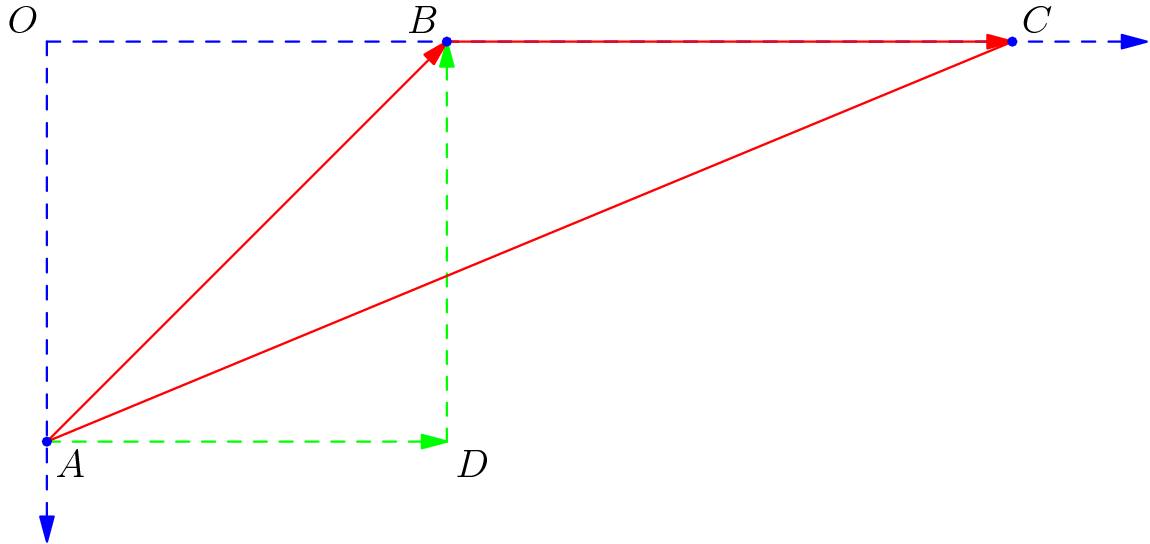
\includegraphics[scale = 0.5]{diagram5.png}
\end{figure}

We also need to do some geometry (see next section).
Let $O$ be the origin.
Let $A$ be the position of the fox.
Let $B$ be the position of the rabbit.
Let $C$ be the intersection of the velocity vectors when extended outwards (this isn't really physically relevant, but we use it later).
Let $D$ be the interesection of the horizontal and vertical components of the fox's velocity (also not physically relevant, but we also use it later).

\subsubsection{Some Geometry}

We start with some angle-chasing.
Let $\angle ABC \equiv \theta$.
By definition of components, $\overline{DB} \perp \overline{AD}$, so $\angle ABD = \theta - \frac{\pi}{2}$.
By complementary angles, $\angle BAD = \frac{\pi}{2} - \angle ABD = \pi - \theta $.
Let $r \equiv \overline{AB}$ and $x \equiv \overline{AD}$.

\subsubsection{Critical Lemma}

We seek to show that throughout the motion, $r+x$ is conserved.
Consider the frame of the rabbit.
In this frame, the fox's horizontal velocity is $ v \cos{\theta}$.
Therefore,

$$\frac{dx}{dt} = v \cos{\theta} - v$$

Now consider the frame of the fox.
In this frame, the rabbit is running away at speed $- v \cos{\theta}$, so

$$ \frac{dr}{dt} = v - v \cos{\theta} $$

Adding the two, we see that

$$\frac{d}{dt} \left (r+x \right) = 0$$

Implying that the quantity is conserved.
Initially, $r+x = a$. After a time $t \gg \frac{a}{v}$ has passed, there is effectively no vertical distance, so $r = x = \frac{a}{2}$.
Notice that we used a conservation law here. Usually, we would have used a standard conservation law, like conservation of energy or momentum, but instead, we made our own conservation law.


\end{document}